\documentclass[times, utf8, seminar, numeric]{fer}
\usepackage{booktabs}
\usepackage{url}
\usepackage{hyperref}
\begin{document}


% TODO: Navedite naslov rada.
\title{Faza konsenzusa u OLC paradigmi sastavljanja genoma – Sparc}

% TODO: Navedite vaše ime i prezime.
\author{Nikola Bukovac, Vinko Kolobara}

% TODO: Navedite ime i prezime voditelja.
\voditelj{Mile Šikić}

\maketitle

\tableofcontents

\chapter{Uvod}
DNK je važna sastavnica svakog živog bića s obzirom da sadrži svu biološku informaciju svake jedinke, što je jedan od razloga zašto ju znanstvenici pokušavaju što preciznije očitati. Današnji uređaji su dovoljno brzi i jeftini, ali problem predstavljaju kratka očitanja koja je moguće napraviti s takvim uređajima, te se stoga razvijaju i algoritmi koji će dobivena očitanja pokušati spojiti u jedan slijed.

Danas je jedna od najraširenijih metoda sekvenciranja genoma takozvana \emph{shotgun} \cite[Poglavlje~1.2.2]{sikic2013bioinformatika} metoda sekvenciranja kod koje se DNK cjepka slučajnim načinom na male dijelove na različitim pozicijama i različitim duljinama. Takav način sekvenciranja dovodi do nepreciznosti samih očitanja DNK pa je taj proces potrebno provoditi nekoliko puta nad istim dijelovima za kvalitetnu rekonstrukciju DNK. Uređaji koji se danas pretežno koriste pripadaju drugoj generaciji uređaja za sekvenciranje, koji iako su jako precizni ostvaruju jako male dužine očitanja, veličine do nekoliko stotina parova nukleotida što značajno usporava sam proces očitavanja. Kako bi se doskočilo ovom problemu, razvijena je treća generacija uređaja koja može očitati od 5 tisuća do 120 tisuća parova nukleotida u jednom čitanju, ali veliki problem predstavlja jako velika pogreška u očitanju koja iznosi od 15\% do 50\%.

Probleme koji nastaju pri očitavanju genoma rješavamo s algoritmima sastavljanja genoma te tako spajamo kraća očitanja i popravljamo nastale greške kod očitanja. Moderni algoritmi koji se bave ovim problemom temelje se na grafovima, a najkorištenije su dvije metode: \emph{Preklapanje-Razmještaj-Konsenzus} metoda temeljena na grafu preklapanja ili metoda temeljena na \emph{k-mer/de Bruijn} grafovima \cite{sikic2013bioinformatika}.

Cilj ovog rada je upoznavanje, implementacija te analiza implementiranog algoritma faze konsenzusa u OLC paradigmi sastavljanja genoma, naziva Sparc. Postavljeni ciljevi nam određuju i samu strukturu rada pa je tako u drugom poglavlju, opisana ideja algoritma Sparc te prikazan grafički primjer koji prikazuje način na koji algoritam radi. Treće poglavlje opisuje kako smo ostvarili našu implementaciju algoritma te što smo sve koristili za nju. Četvrto poglavlje donosi našu analizu rješenja koje smo implementirali te način na koji smo proveli analizu.

%=========================================================================
%Početak drugog poglavlja
%=========================================================================

\chapter{Sparc algoritam}
Algoritam Sparc je algoritam faze konsenzusa u Preklapanje-Razmještanje-Konzenzus (engl. \emph{Overlap-Layout-Consensus, OLC}) paradigmi sastavljanja očitanja genoma. Temelj algoritma se zasniva na \emph{de Bruijn/k-mer} grafu nad kojim se potom provodi ostatak algoritma \cite{Ye2016}.
\section{Opis algoritma}
Prvi korak algoritma je konstrukcija k-mer grafa na temelju predanog ulaza koji sadrži izlaz iz faze Razmještaja, OLC paradigme. Ovisno o parametrima \emph{k} i \emph{g} kreira se inicijalni k-mer graf, gdje navedeni parametri određuju strukturu grafa, konkretno \emph{k} specificira koliko će nukleotida biti sadržano u pojedinom čvoru grafa, a \emph{g} specificira koliko će se nukleotida nalaziti na svakom bridu. Inicijalni graf je usmjeren sa samo jednim bridom iz svakog vrha osim završnog, koji ga nema. Razlika između ovog grafa i klasičnog de Bruijn grafa je u to tome što su isti k-meri na različitim pozicijama nezavisni jedni od drugih dok su kod de Bruijn grafa smješteni u jednom vrhu pa se ovaj graf smatra \emph {sparse} grafom. 

Sljedeći korak algoritma je poravnanje dodatnih slijedova čiji se postupak provodi ovisno o tome odgovara li k-mer u novom slijedu, k-meru u originalnom slijedu i njegovom bridu gdje se onda samo poveća težina brida za definiranu vrijednost, ili ukoliko ne odgovara dodaje se novi brid u graf i kreira se dodatni k-mer i samim time kreira novi put u grafu. Ovaj postupak je jako sličan kreiranju de Bruijn grafa, ali zbog razlikovanja istih k-mera ovisno o njihovoj poziciji, postoji razlika u postupku. Ovaj korak se ponavlja za sve slijedove koje smo dobili sekvenciranjem. 

Završni korak Sparc algoritma je traženje puta u grafu koji ima najveću težinu, što je zahvaljujući činjenici da je konstruirani graf usmjeren i acikličan moguće napraviti s BFS ili DFS algoritmom kojim računamo težinu svakog vrha u grafu. Određivanje konsenzusnog slijeda se provodi tako da krenemo od najtežeg vrha i vraćamo se po najvećim težinama natrag sve do početnog vrha.

\section{Primjer}
\begin{figure}[htb]
	\centering
	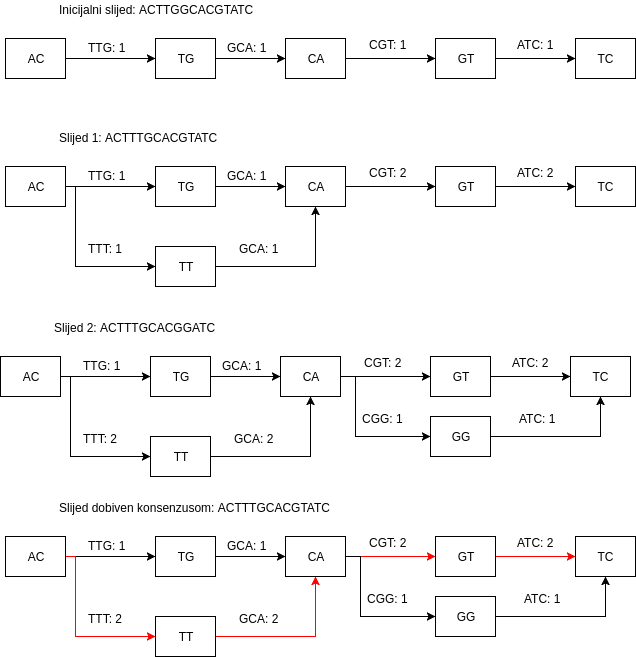
\includegraphics[scale=0.6]{images/backbone.png}
	\caption{Postupak izgradnje grafa s k=2, g=3}
	\label{picture:example}
\end{figure}

Slika \ref{picture:example} prikazuje cjelokupni postupak algoritma Sparc. Inicijalni slijed služi za kreiranje inicijalnog lanca (engl. \emph{backbone}). Nakon kreiranja \emph{backbone}-a grafa, sljedeći slijed poravnavamo tako da krećemo od početka slijeda i vidimo da je prvi k-mer AC jednak k-meru konstruiranom u grafu, ali je prijelaz na sljedeći k-mer TTT različit od onoga koji se nalazi u grafu te je stoga potrebno konstruirati novi k-mer TT te novi brid iz k-mera AC prema novom k-meru TT, a taj brid je TTT. Sljedećih \emph{g} nukleotida je GCA koji trebaju završiti u k-meru CA koji već postoji u konstruiranom grafu te je potrebno kreirati brid CGA od k-mera TT prema k-meru CA. Sljedećih \emph{g} nukleotida je CGT, budući da taj brid postoji u konstruiranom grafu potrebno je samo povećati težinu postojećeg brida, isto vrijedi i za sljedećih \emph{g} nukleotida ATC. Postupak je jednak i za slijed 2. Za određivanje najtežeg puta pratimo bridove s najvećim težinama, a u ovdje kontruiranom grafu to je put od k-mera AC bridom TTT potom bridom GCA, CGT i ATC te je stoga rekonstruirani slijed ACTTTGCACGTATC.

%=======================================================================
%Početak trećeg poglavlja
%=======================================================================

\chapter{Naša implementacija algoritma}
Za ostvarivanje naše implementacije algoritma faze konzensuza Sparc, koristili smo programski jezik C++ uz korištenje dodatnih biblioteka i alata, koji će biti navedeni u nastavku. Implementacija koristi specifične formate podataka koji su također opisani u nastavku.
\section{Korišteni formati podataka}
Svi podaci o slijedovima koje koristimo u našem algoritmu nalaze se u predodređenim formatima podataka kako bi se algoritam mogao što jednostavnije koristiti u opće svrhe. 
\subsection{FASTA}
Naš algoritam ovaj format koristi kako bi napravio početni lanac (engl. \emph{backbone}), za ulaz te na izlaz stavlja rekonstruirani slijed također u FASTA formatu.
Ulaz u naš algoritam je u biti izlaz iz faze razmještaja OLC paradigme \cite[Poglavlje~1.3.1]{sikic2013bioinformatika}.
\subsection{FASTQ}
Sličan FASTA formatu, ali osim samog slijeda sadrži i oznaku kvalitete svakog očitanja.
Ovaj format podataka sadrži sekvencirane slijedove koji će poslužiti za rekonstrukciju originalnog slijeda \cite[Poglavlje~1.3.2]{sikic2013bioinformatika} .
Iako naša implementacija ne koristi direktno ovaj format podataka, on se koristi kao ulaz za alat GraphMap koji služi za generiranje SAM formata podataka. 
\subsection{SAM}
Ovaj format podataka sadrži grupirane informacije o svim očitanjima iz FASTQ formata podataka \cite{sam_format}. Podaci iz ovog formata podataka služe za rekonstrukciju genoma. 

Podaci iz SAM formata podataka koje koristimo u našoj implementaciji su:
\renewcommand{\labelitemi}{$\bullet$}
\begin{itemize}
	\item FLAG - skup zastavica koje ovisno o vrijednosti utječu na naš algoritam. Vrijednost zastavice 4 označava da je trenutno mapiranje nepostojeće te stoga preskačemo mapiranje, također uzimamo u obzir i vrijednost zastavice 16 koja označava da je trenutni slijed u SEQ dijelu inverzno komplementiran. Ostale vrijednosti zastavica zanemarujemo.  
	\item POS - pozicija na osnovnom slijedu na kojoj počinje trenutno mapiranje, pozicija je indeksirana od indeksa 1
	\item CIGAR - popis operacija koje su napravljene nad očitanjem kako bi se dobilo mapiranje
	\item SEQ - originalno očitan slijed, prije nego što su obavljene CIGAR operacije
	\item QUAL - ASCII string u \emph{Phred} bazi, definira kvalitetu mapiranja
\end{itemize}

\section{Korištene biblioteke}
Osim standardnih biblioteka programskog jezika C++, kao što su na primjer biblioteke za I/O operacije te STL(\emph{Standard Template Library}) biblioteke koja sadrži implementacije složenijih struktura podataka, koristili smo i biblioteku/alat GraphMap.
\subsection{GraphMap} 
GraphMap \cite{graphmap} biblioteka pruža implementaciju mapiranja poravnanja očitanih slijedova u odnosu na početni slijed. Ovu biblioteku smo koristili kako bi dobili poravnanja slijedova koja onda koristimo kod Sparc algoritma za konstruiranje grafa. Mapiranja poravnanja se dobiju tako što se GraphMap alatu predaju slijed na kojem želimo raditi poravnanje u FASTA formatu te datoteku s očitanjima slijedova u FASTQ formatu. Korištenjem opcije \emph{align} dobiju se mapiranja poravnanja u SAM formatu datoteke.

GraphMap alat nismo koristili direktno u našoj implementaciji, ali smo koristili nastala mapiranja kako bi napravili što efikasniji algoritam.

\section{Struktura implementacije}
Implementacija je raspodijeljena na nekoliko cjelina: glavni program, definicije formata podataka i njihove parsere te dio u kojemu je definirana struktura k-mer grafa kao i implementacija samog Sparc algoritma.

Datoteka \emph{main.cpp} predstavlja glavni program u kojemu se instanciraju potrebne klase za provedbu algoritma kao i svi potrebni parseri koje koristimo.

Definicije svih formata datoteka se nalaze u direktoriju \emph{format} gdje je za svaki format podataka napravljena \emph{header} datoteka i njena implementacija.

Implementacija samoga algoritma se nalazi u direktoriju \emph{algorithm} gdje je također napravljena \emph{header} datoteka i njena implementacija. Sparc se nalazi u razredu \emph{KMerGraph} koji predstavlja implementaciju k-mer grafa, dok strukture \emph{Vertex} i \emph{Edge} predstavljaju reprezentacije vrha te brida grafa. Kod instanciranja razreda \emph{KMerGraph} predaju se parametri \emph{k} i \emph{g} kojima se definira struktura grafa, a sama izgradnja \emph{backbone-a} se provodi s metodom \emph{initialGraph} kojoj se predaje \emph{layout} dobiven iz faze Razmještaja. Nakon izgradnje početnog grafa prolazimo po datoteci SAM formata koja sadrži podatke o obavljenim mapiranjima poravnanja na osnovni slijed. Pomoću dobivenih mapiranja gdje su nam najvažnije stavke originalni slijed \emph{SEQ} prije \emph{CIGAR} operacija, same \emph{CIGAR} operacije, početna pozicija u poravnanju te kvaliteta mapiranja, radimo dodavanje na početni graf bilo povećavanjem težina postojećih bridova ili dodavanjem novih bridova i k-mera. Težine bridova se povećavaju za vrijednost koja se dobije izračunom prosjeka iz vrijednosti \emph{QUAL} i \emph{g}, čime radimo prosječnu vrijednost \emph{QUAL} po broju nukleotida na bridu. Nakon čitanja cijele SAM datoteke pokreće se traženje najtežeg puta u grafu i određivanje konsenzusnog slijeda koji je definiran najtežim putem u grafu.

\section{Instalacija i pokretanje algoritma}
Cjelokupna implementacija je javno dostupna na poslužitelju GitHub na poveznici \url{https://github.com/vkolobara/bioinf}. Za instalaciju je potrebno ili klonirati postojeći repozitorij ili skinuti \emph{.zip} arhivu te pokrenuti skriptu \emph{install.sh} kako bi se povukle sve potrebne biblioteke i testni podaci te preveli izvorni kodovi u izvršne datoteke. 

Pokretanje algoritma se provodi pokretanjem skripte \emph{run.sh} kojoj je moguće predati dodatne parametre koji specificiraju parametre \emph{k} i \emph{g} te broj iteracija i naziv testne datoteke koju želimo pokrenuti.

%===========================================================================
% Početak četvrtog poglavlja
%==========================================================================

\chapter{Analiza implementacije}
Za utvrđivanje kvalitete implementacije, radimo usporedbu slijeda koji smo koristili kao ulaz u algoritam te konsenzusnog slijeda kojeg smo dobili kao izlaz iz algoritma s referentnim slijedom. Usporedbu radimo pomoću DnaDiff \cite{MUMMER} alata koji nam pruža informaciju koliki je postotak podudarnosti našeg i referentnog slijeda. Postotak podudarnosti slijedova nam je najbitniji podatak prilikom analize, ali jednako tako su nam važni i podaci o utrošku memorijskog prostora te vremenu izvođenja algoritma.

\section{Alati za analizu}
Kako bi analiza podataka bila što preciznija koristimo gotove alate, kojima provjeravamo prije navedene čimbenike koje pratimo.

\subsection{DnaDiff}
DnaDiff \cite{MUMMER} je jedan od alata iz programskog paketa otvorenog koda MUMmer, koji osim alata DnaDiff sadrži i druge alate koji se koriste na području bioinformatike. DnaDiff radi analizu između dva genetska slijeda i utvrđuje njihovu sličnost. Analiza provedena alatom daje detaljne informacije o sličnostima slijedova, ali kao faktor kvalitete implementacije smo koristili podatke iz datoteke \emph{out.report} i poglavlja o sličnosti poravnanja, \emph{Alignments}. Navedeno poglavlje ima analizu za 1-1 i M-M poravnanja koja su prilikom naših testiranja u većini slučajeva za polje AvgIdentity bila identične ili gotovo identične vrijednosti pa smo stoga kao faktor kvalitete rješenja odlučili koristiti vrijednost pod 1-1 AvgIdentity.

\subsection{cgmemtime}
Alat cgmemtime \cite{cgmemtime} služi za analizu vremena i potrošene memorije. Za memoriju se ispisuje najveća zabilježena vrijednost za vrijeme izvođenja algoritma te tako imamo informaciju koliko je minimalno memorije potrebno rezervirati za izvođenje programa.


\section{Testna konfiguracija}
Osnovni podaci o računalnoj konfiguraciji koja je korištena za analizu izvođenja ostvarenog rješenja navedena je u nastavku:
\renewcommand{\labelitemi}{$\bullet$}
\begin{itemize}
	\item Operacijski sustav - Arch Linux x86 64
	\item Procesor - Intel Core i3-6100 @ 3.70GHz
	\item RAM - 16 GiB DDR4 @ 2133MHz
\end{itemize}

\section{Analiza kvalitete rješenja}
\begin{table}[htb]
	\centering
	\begin{tabular}{l|ccc}
		& \multicolumn{1}{l}{k} &g 		&vrijednost\\ 	\hline
		 	1			&1	 	&1 		& 88.93 \\ 		\hline
		 	2			&1	 	&2		& 90.19 \\ 		\hline
		 	3			&1	 	&3 		& 89.32 \\ 		\hline
		 	4			&1	 	&4 		& 90.67 \\ 		\hline
		 	5			&1	 	&5 		& 89.74 \\ 		\hline
		 	6			&2	 	&3 		& 88.86 \\ 		\hline
		 	7			&2	 	&4		& 90.64 \\ 		\hline
		 	8			&2	 	&5		& 89.70 \\ 		\hline
		 	9			&2	 	&6 		& 90.19 \\ 		\hline
		 	10			&3	 	&4 		& 90.94 \\ 		\hline
		 	11			&3	 	&5 		& 89.78 \\ 		\hline
		 	12			&3	 	&6 		& 89.92 \\ 		\hline
		 	13			&4	 	&5 		& 89.85 \\ 		\hline
		 	14			&3		&2		& 90.19 \\		\hline
		 	15			&4		&2		& 90.11	\\		\hline
	\end{tabular}
	\caption{Testiranje algoritma za različite vrijednosti parametara k i g na testnom skupu lambda za jednu iteraciju}
	\label{table:lambda_test}
\end{table}

Tablica \ref{table:lambda_test} prikazuje kretanje vrijednosti podudarnosti slijeda dobivenog algoritmom i referentnog slijeda. Moguće je primijetiti da se najbolja rješenja pronalaze za vrijednosti parametara \emph{k} = 3 i \emph{g} = 4, te su stoga te vrijednosti korištene za daljnju analizu na drugim testnim skupovima.

\begin{table}[htb]
	\centering
	\begin{tabular}{l|c}
		& \multicolumn{1}{l}{vrijednost}\\ 	\hline
		1. 					& 90.95 	\\ 	\hline
		2.  				& 91.47 	\\	\hline
		3.		   			& 91.67		\\ 	\hline
		4.		   			& 91.78		\\ 	\hline
		5.		   			& 91.85		\\ 	\hline
	\end{tabular}
	\caption{Promjena vrijednosti kvalitete kroz više iteracija za k=3 i g=4 na testnom skupu lambda.}
	\label{table:iteracije}
\end{table}


Tablica \ref{table:iteracije} prikazuje kako se uz korištenje više iteracija algoritma, na način da se izlaz iz iteracije \emph{i} koristi kao ulaz u iteraciji \emph{i+1}, moguće poboljšati kvalitetu poklapanja između referentnog slijeda i našeg konsenzusnog slijeda. Također je vidljivo da više iteracije donose sve manja poboljšanja u odnosu na prethodne.

\begin{table}[htb]
	\centering
	\begin{tabular}{l|cc}
		& \multicolumn{1}{l}{lambda} & ecoli \\ 	\hline
		layout 					& 86.16 	& 88.57 \\ 	\hline
		naš  					& 91.85     & 95.87 \\	\hline
		original		   		& 96.83 	& 99.01 \\ 	\hline
	\end{tabular}
	\caption{Usporedba naše implementacije sa slijedom iz faze razmještanja (layout) i referentnim radom (Sparc) za k=3 i g=4.}
	\label{table:kvaliteta}
\end{table}

Tablica \ref{table:kvaliteta} prikazuje usporedbu naše implementacije i implementacije referentnog rada iz koje je vidljivo da implementacija iz referentnog rada dobiva bolja rješenja od našeg algoritma, iako oba rješenja uspijevaju poboljšati slijed iz faze Razmještaj.
Tijekom testiranja našeg algoritma primijetili smo da najbolje rezultate dobivamo upravo za ovakve postavke parametara \emph{k} i \emph{g}. 

Referentni rad navodi da su optimalni parametri za taj algoritam \emph{k} u rasponu od 1 do 2 te \emph{g} u rasponu od 1 do 3. 

\section{Analiza utroška memorije i vremena}
\begin{table}[htb]
	\centering
	\begin{tabular}{l|cc}
		& \multicolumn{1}{l}{vrijeme[s]} & memorija[MiB] \\ 	\hline
		lambda			& 0.17		& 20 	\\ 	\hline
		ecoli  			& 26.8     	& 1600  \\	\hline
	\end{tabular}
	\caption{Analiza utroška vremena i memorije za provedbu algoritma za k=3 i g=4.}
	\label{table:memorija}
\end{table}

Tablica \ref{table:memorija} prikazuje potrošnju memorije i vrijeme izvođenja naše implementacije algoritma i iz nje je moguće vidjeti da su zadovoljena zadana ograničenja za oba skupa podataka. 

%=====================================================================
% Ostatak poglavlja
%=====================================================================

\chapter{Zaključak}
Paradigma Premještaj-Razmještaj-Konsenzus pruža jedan način rješavanja problema sastavljanja genoma poslije njihovog sekvenciranja i radom na ovom projektu imali smo priliku implementirati jedan od algoritama koji se bave ovim problemom. Implementirani algoritam spada u fazu konsenzusa spomenute paradigme i naziva se Sparc, algoritam je temeljen na k-mer grafovima te zbog toga spada u modernije načine rješavanja sastavljanja genoma.

Tijekom implementacije smo radili i analizu kvalitete rješenja na dostupnim testnim skupovima i ovisno o rezultatima smo prilagođavali implementaciju. Nakon što smo pronašli zadovoljavajuće parametre radili smo usporedbu s referentnim algoritmom i utvrdili da iako oba algoritma poboljšavaju početni slijed, referentni algoritam to radi bolje.


\bibliography{literatura}
% Ukljuci literaturu u seminar
\nocite{*}
\bibliographystyle{fer}

\chapter{Sažetak}
Algoritam Sparc je jedna od implementacija algoritma faze konsenzusa u Premještaj-Razmještaj-Konsenzus paradigmi sastavljanja genoma. 
Navedeni algoritam je implementiran u ovom projektu te je dodatno provedena analiza kvalitete rješenja s gotovim alatima, te je također napravljena usporedna analiza s originalnom implementacijom koja je napravljena u referentnom radu. Naša implementacija uspijeva propraviti početni slijed, ali ne u takvoj mjeri kao što to uspijeva originalna implementacija.

\end{document}
